\documentclass[12pt]{article}
\usepackage[margin=1in]{geometry} 
\usepackage{graphicx}
\usepackage{amsmath,amsthm,amssymb}
\usepackage{hyperref}
\usepackage{listings}
\usepackage{tcolorbox}

\title{
    \textbf{CS5280: Project Report} \\
    \textbf{Concurrent Execution of Blockchain Smart Contract transactions (SCTs)} \\ 
}

% \author{
%     \textbf{Darpan Gaur} \\
%     \textbf{CO21BTECH11004}
% }
% write two authors in two columns
\author{
    \begin{tabular}{c}
        \textbf{Darpan Gaur} \\
        \textbf{CO21BTECH11004}
    \end{tabular}
    \begin{tabular}{c}
        \textbf{Yoshita Kondapalli} \\
        \textbf{CO21BTECH11008}
    \end{tabular}
}

% Define the style for the code box
\tcbuselibrary{listings, breakable, skins}
\lstset
{ %Formatting for code in appendix
    language=C++,
    basicstyle=\footnotesize,
    numbers=left,
    stepnumber=1,
    showstringspaces=false,
    tabsize=1,
    breaklines=true,
    breakatwhitespace=false,
}
\tcbset{
    colback=white,
    colframe=black!70,
    listing only,
    left=5mm,
    enhanced,
    boxrule=0.5pt,
    top=0pt,
    bottom=0pt,
    sharp corners,
    breakable,
    listing options={
        basicstyle=\small\ttfamily,
        numbers=left,
        numberstyle=\tiny\color{gray},
        breaklines=true,
        language=C++,
        captionpos=b,
        label=lst:example
    }
}

\date{}

\begin{document}
\maketitle

\hrulefill

\section{Problem Statement}
Sequential execution of smart contract transactions (SCTs) in blockchain systems restricts concurrency and limits performance.
There is a need for a framework that facilitates concurrent execution of SCTs, enhancing performance by allowing non-conflicting transactions to be processed simultaneously while preserving deterministic order.
In this project, we aim to compare two frameworks: \textbf{DAG} and \textbf{BlockPilot}, which enable parallel execution of SCTs. We will implement these frameworks and evaluate their performance based on execution time, abort rates, and scalability.

\section{DAG}

In blockchain systems, particularly those handling smart contracts, executing transactions sequentially within a block limits throughput and scalability. To address this, they employ a DAG-based (Directed Acyclic Graph) parallel execution framework. The DAG encodes dependencies between transactions based on their read and write sets, ensuring that only independent transactions are executed concurrently. This approach allows for a significant improvement in execution efficiency.

The DAG represents transactions as nodes and dependencies (conflicts) as directed edges. A transaction $T_i$ has an edge to $T_j$ if $T_j$ accesses data that $T_i$ modifies or vice versa. Three types of conflicts are considered:
\begin{itemize}
    \item Read-Write conflict: $T_i$ writes to an address that $T_j$ reads.
    \item Write-Read conflict: $T_i$ reads from an address that $T_j$ writes to.
    \item Write-Write conflict: Both $T_i$ and $T_j$ write to the same address.
\end{itemize}

Only transactions with zero incoming edges (i.e., no unresolved dependencies) can be safely executed in parallel. After executing a transaction, its outgoing edges are removed (i.e., dependent transactions' in-degree is decremented), allowing other transactions to become eligible for execution.

\section{Design of DAG}

Our implementation consists of two main phases: DAG construction and parallel transaction execution. The design is modular, thread-safe, and optimized for performance.

\subsection{DAG Construction}

The DAG is constructed using multiple threads to parse a list of transactions read from an input file. Each transaction consists of a read set and a write set. The DAG is represented using an adjacency list and an atomic array for in-degree counts. The construction process proceeds as follows:

\begin{enumerate}
    \item Each thread picks the next transaction index to process using an atomic counter.
    \item For each transaction $T_i$, all subsequent transactions $T_j$ are checked for conflicts:
    \begin{itemize}
        \item If any address in $T_i$'s write set intersects with $T_j$'s read or write set, or
        \item If any address in $T_i$'s read set intersects with $T_j$'s write set,
    \end{itemize}
    then an edge is added from $T_i$ to $T_j$, and the in-degree of $T_j$ is incremented.
\end{enumerate}

\subsection{Parallel Execution}

Transaction execution is also handled in parallel by multiple threads. Each thread selects a transaction with zero in-degree (i.e., no pending dependencies) using a two-pass scan over the DAG. The `compare\_exchange` operation ensures atomicity and prevents duplicate execution. Once a transaction is selected:
\begin{enumerate}
    \item It is executed (simulated in our implementation),
    \item Its successors' in-degrees are decremented,
    \item The process repeats until all transactions are executed.
\end{enumerate}

\subsection{Implementation Details}

Our DAG and scheduler are implemented in C++ for concurrency efficiency. Key implementation details include:
\begin{itemize}
    \item A vector of atomic integers for in-degrees.
    \item An adjacency list using vectors.
    \item Use of mutexes to control file output access across threads.
    \item Thread-safe DAG construction and transaction execution using atomic counters and synchronization.
\end{itemize}

\subsection{Benefits}

This design aligns with the framework proposed in \textit{Piduguralla et al. (2023)} and yields significant improvements in throughput compared to serial and tree-based execution models. The adjacency matrix version used here is more performant due to direct access and reduced pointer traversal overhead.





\section{Block Pilot}

In modern blockchain systems, transaction throughput remains limited by serial execution, especially when validators and proposers operate under different execution contexts. \textbf{BlockPilot} addresses this issue by enabling parallel execution of smart contract transactions (SCTs) across both proposer and validator roles. It introduces an \textit{Optimistic Concurrency Control with Write Snapshot Isolation (OCC-WSI)} algorithm for proposers, and a \textit{pipeline scheduling framework} for validators.

In our implementation inspired by BlockPilot, we adopt a proposer-style OCC-WSI mechanism, enabling each thread to execute transactions based on a consistent snapshot and verify for conflicts post-execution. A transaction is committed if no conflicting version updates occurred since its snapshot; otherwise, it is aborted and retried.

Validators execute the committed transactions from the proposed block using a dependency-based parallel scheduler. The scheduler builds a conflict graph and assigns transactions with no interdependencies to different threads, executing subgraphs concurrently while preserving the serial order within each subgraph.

This design enables efficient, parallel execution of SCTs while preserving deterministic execution outcomes, essential for consensus and fault tolerance in blockchain.


\section{Correctness of Snapshot Isolation}


\section{Design of Block Pilot}

Our implementation draws directly from the BlockPilot architecture, employing an \textit{OCC-WSI concurrency protocol} and a \textit{thread-based parallel scheduler}. The execution design is comprised of the following core components:

\subsection*{Proposer-Side: OCC-WSI Execution}

The proposer initializes a reserve table to track versioning for each data item and assigns each transaction a \texttt{snapshot version}. The algorithm proceeds as follows:
\begin{enumerate}
    \item Each thread selects an available transaction using atomic operations.
    \item The transaction reads from a consistent snapshot of the data state.
    \item Execution is performed in a local memory buffer (read set and write set).
    \item A conflict detection step checks if any data read has been modified since the snapshot version.
    \item If validation passes, the transaction's write set is committed, and the reserve table is updated.
    \item If validation fails, the transaction is aborted and may be retried.
\end{enumerate}

This behavior mirrors Algorithm 1 in BlockPilot, and the core logic is implemented in our \texttt{detectConflict()} method in \texttt{scheduler.cpp}.

Pseudo code for the OCC-WSI execution is provided in Listing \ref{lst:occ-wsi}.

\begin{tcolorbox}
\begin{lstlisting}[language=C++, caption={Pseudo code for OCC-WSI Execution}, label={lst:occ-wsi}]
void threadFunc(int threadID) {
    while (completedTxn < totTrans) {
        int txnID = selectTxn();

        snapshotVersion = state;

        rs, ws = executeTx(txnID, snapshotVersion);

        conflictResult = detectConflict(txnID, rs, ws);
        if (conflictResult == -1) {
            // Transaction aborted
            continue;
        }
        // Transaction committed
        completedTxn++;
    }
}

int detectConflict(int txnID, set<int> rs, set<int> ws) {
    for (int rec: rs) {
        if (Table[rec] > snapshotVersion) {
            // Conflict detected
            return -1;
        }
        
    }
    state = snapshotVersion + 1;
    for (int rec: ws) {
        Table[rec] = state;
        // update the global memory
    }
    return 0;   // transaction committed
}

\end{lstlisting}
\end{tcolorbox}



\section{Transaction Generator}
The purpose of this program is to generate a specified number of random transactions consisting of read/write operations on multiple accounts. It ensures that the generated transactions match a desired level of dependency (conflict) between them and saves them to a file.

\subsection*{6.1 Inputs}
The program takes the following inputs from the user:
\begin{itemize}
    \item \textbf{Target Dependency Percentage (0--100)}: Desired percentage of conflicting transaction pairs.
    \item \textbf{Number of Transactions ($\geq$ 2)}: Total number of transactions to generate.
    \item \textbf{Number of Accounts ($\geq$ 1)}: Number of accounts on which operations are performed.
\end{itemize}

\subsection*{6.2 Core Functionalities}

\subsection*{\texttt{generate\_transaction(num\_accounts)}}
Generates a single transaction consisting of 1 to 3 random operations. Each operation is randomly selected as a read (\texttt{r}) or write (\texttt{w}) on a randomly chosen account.

\subsection*{\texttt{generate\_transactions(num\_transactions, num\_accounts)}}
Generates a list of transactions by calling \texttt{generate\_transaction} repeatedly.

\subsection*{\texttt{transaction\_has\_conflict(t1, t2)}}
Determines whether two transactions conflict. A conflict exists if both access the same account and at least one operation is a write.

\subsection*{\texttt{calculate\_dependency(transactions)}}
Calculates the percentage of conflicting transaction pairs. It uses the formula:
\[
\text{Dependency (\%)} = \frac{\text{Number of Conflicting Pairs}}{\binom{n}{2}} \times 100
\]
where $n$ is the number of transactions.

\subsection*{\texttt{save\_transactions(transactions, filename)}}
Saves the transactions to a text file in the format \texttt{r(1), w(2), r(3)}.

\subsection*{6.3 Execution Flow}

\subsubsection*{Input Validation}
The program prompts the user for valid numeric inputs that meet the following constraints:
\begin{itemize}
    \item Target dependency percentage must be between 0 and 100.
    \item Number of transactions must be at least 2.
    \item Number of accounts must be at least 1.
\end{itemize}

\subsubsection*{Attempt Loop}
The program makes up to 5 attempts to generate a set of transactions that meets the target dependency percentage within a tolerance of $\pm$1\%. On a successful attempt:
\begin{itemize}
    \item The transactions are saved to \texttt{transactions.txt}.
    \item Dependency percentage and attempt details are printed to the console.
\end{itemize}

If none of the attempts succeed, a failure message is displayed after all 5 tries.

\subsubsection*{Output}
\begin{itemize}
    \item \textbf{File Output:} \texttt{transactions.txt}, containing the list of generated transactions.
    \item \textbf{Console Output:} Displays success/failure messages, attempt number, and achieved dependency.
\end{itemize}

\subsubsection*{Example Output}
For 5 transactions and 3 accounts, a possible output is:
\begin{verbatim}
r(1), w(3)
w(2), r(3)
r(1)
w(2), w(1)
r(2), w(3)
\end{verbatim}

Dependency achieved: 70\% (Target: 70\%)


\section{Experiments}
\subsection{Number of Transactions}
In this experiment number of transactions are varied from 1000 to 5000 in increments of 1000. 
The number of threads is kept constant at 16 and dependency percentage is kept constant at 40\%. \\
Figure \ref{fig:numTrans_vs_Time} shows the execution time vs number of transactions and Figure \ref{fig:numTrans_vs_Aborts} shows the number of aborts vs number of transactions.
Figure \ref{fig:numTrans_vs_DAGCreationTime} shows the DAG creation time vs number of transactions.
For DAG time to execute the transactions is taken and reported in figure, DAG creation time is not included. 
\begin{itemize}
    \item As number of transactions increases, the execution time also increases.
    \item Block Pilot performs better than DAG in terms of execution time.
    \item Number of aborts also increases with the number of transactions.
    \item DAG creation time also increases with the number of transactions.
\end{itemize}

\begin{figure}[h]
    \centering
    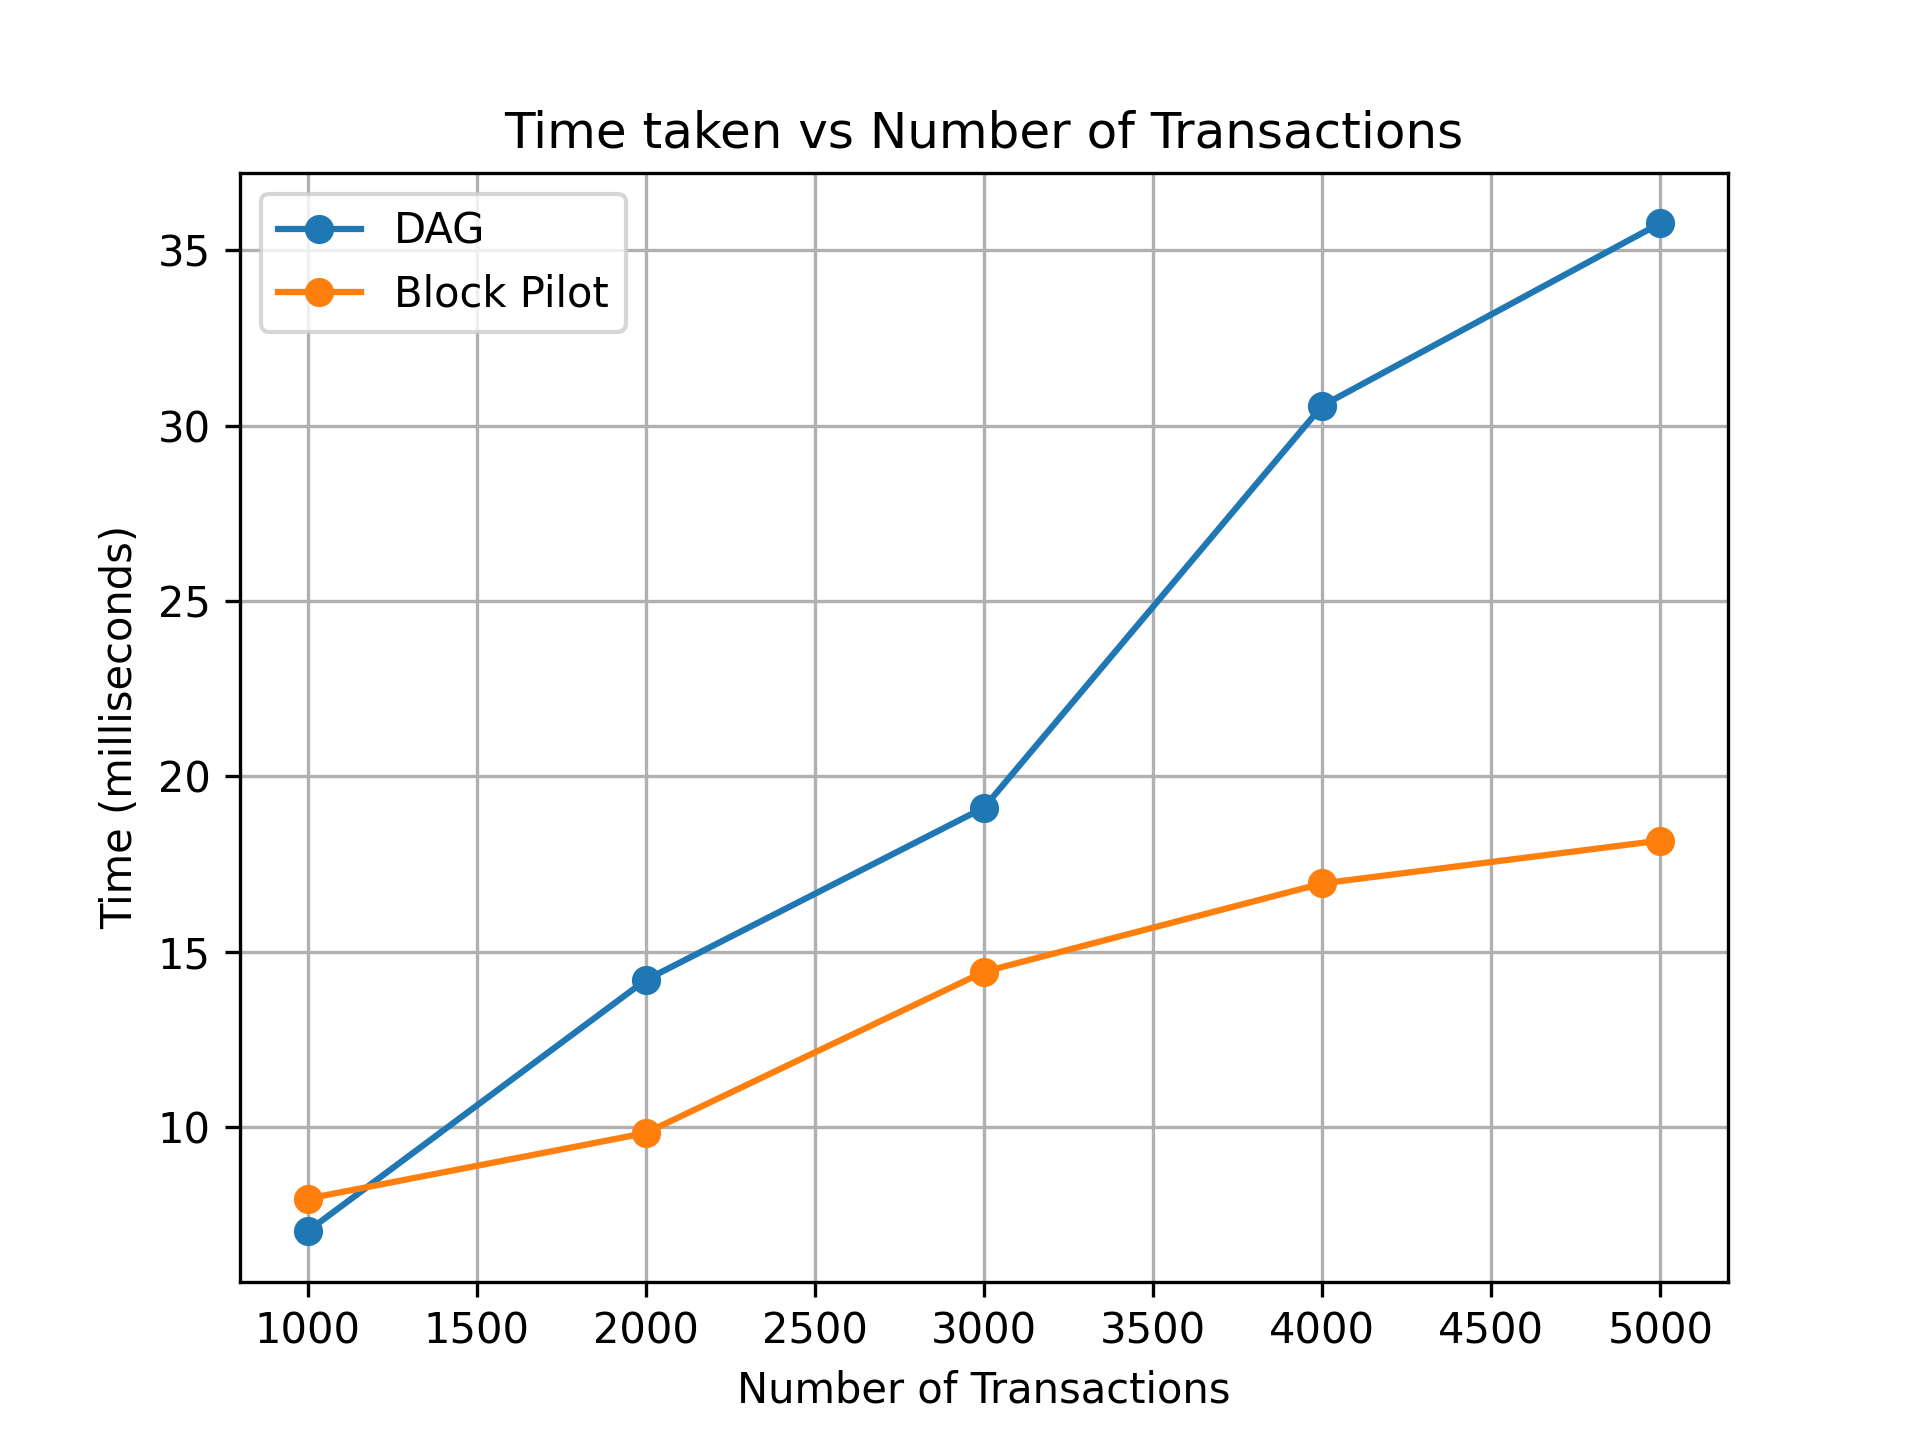
\includegraphics[width=0.8\textwidth]{images/numTrans_vs_Time.png}
    \caption{Execution Time vs Number of Transactions}
    \label{fig:numTrans_vs_Time}
\end{figure}

\begin{figure}[h]
    \centering
    % 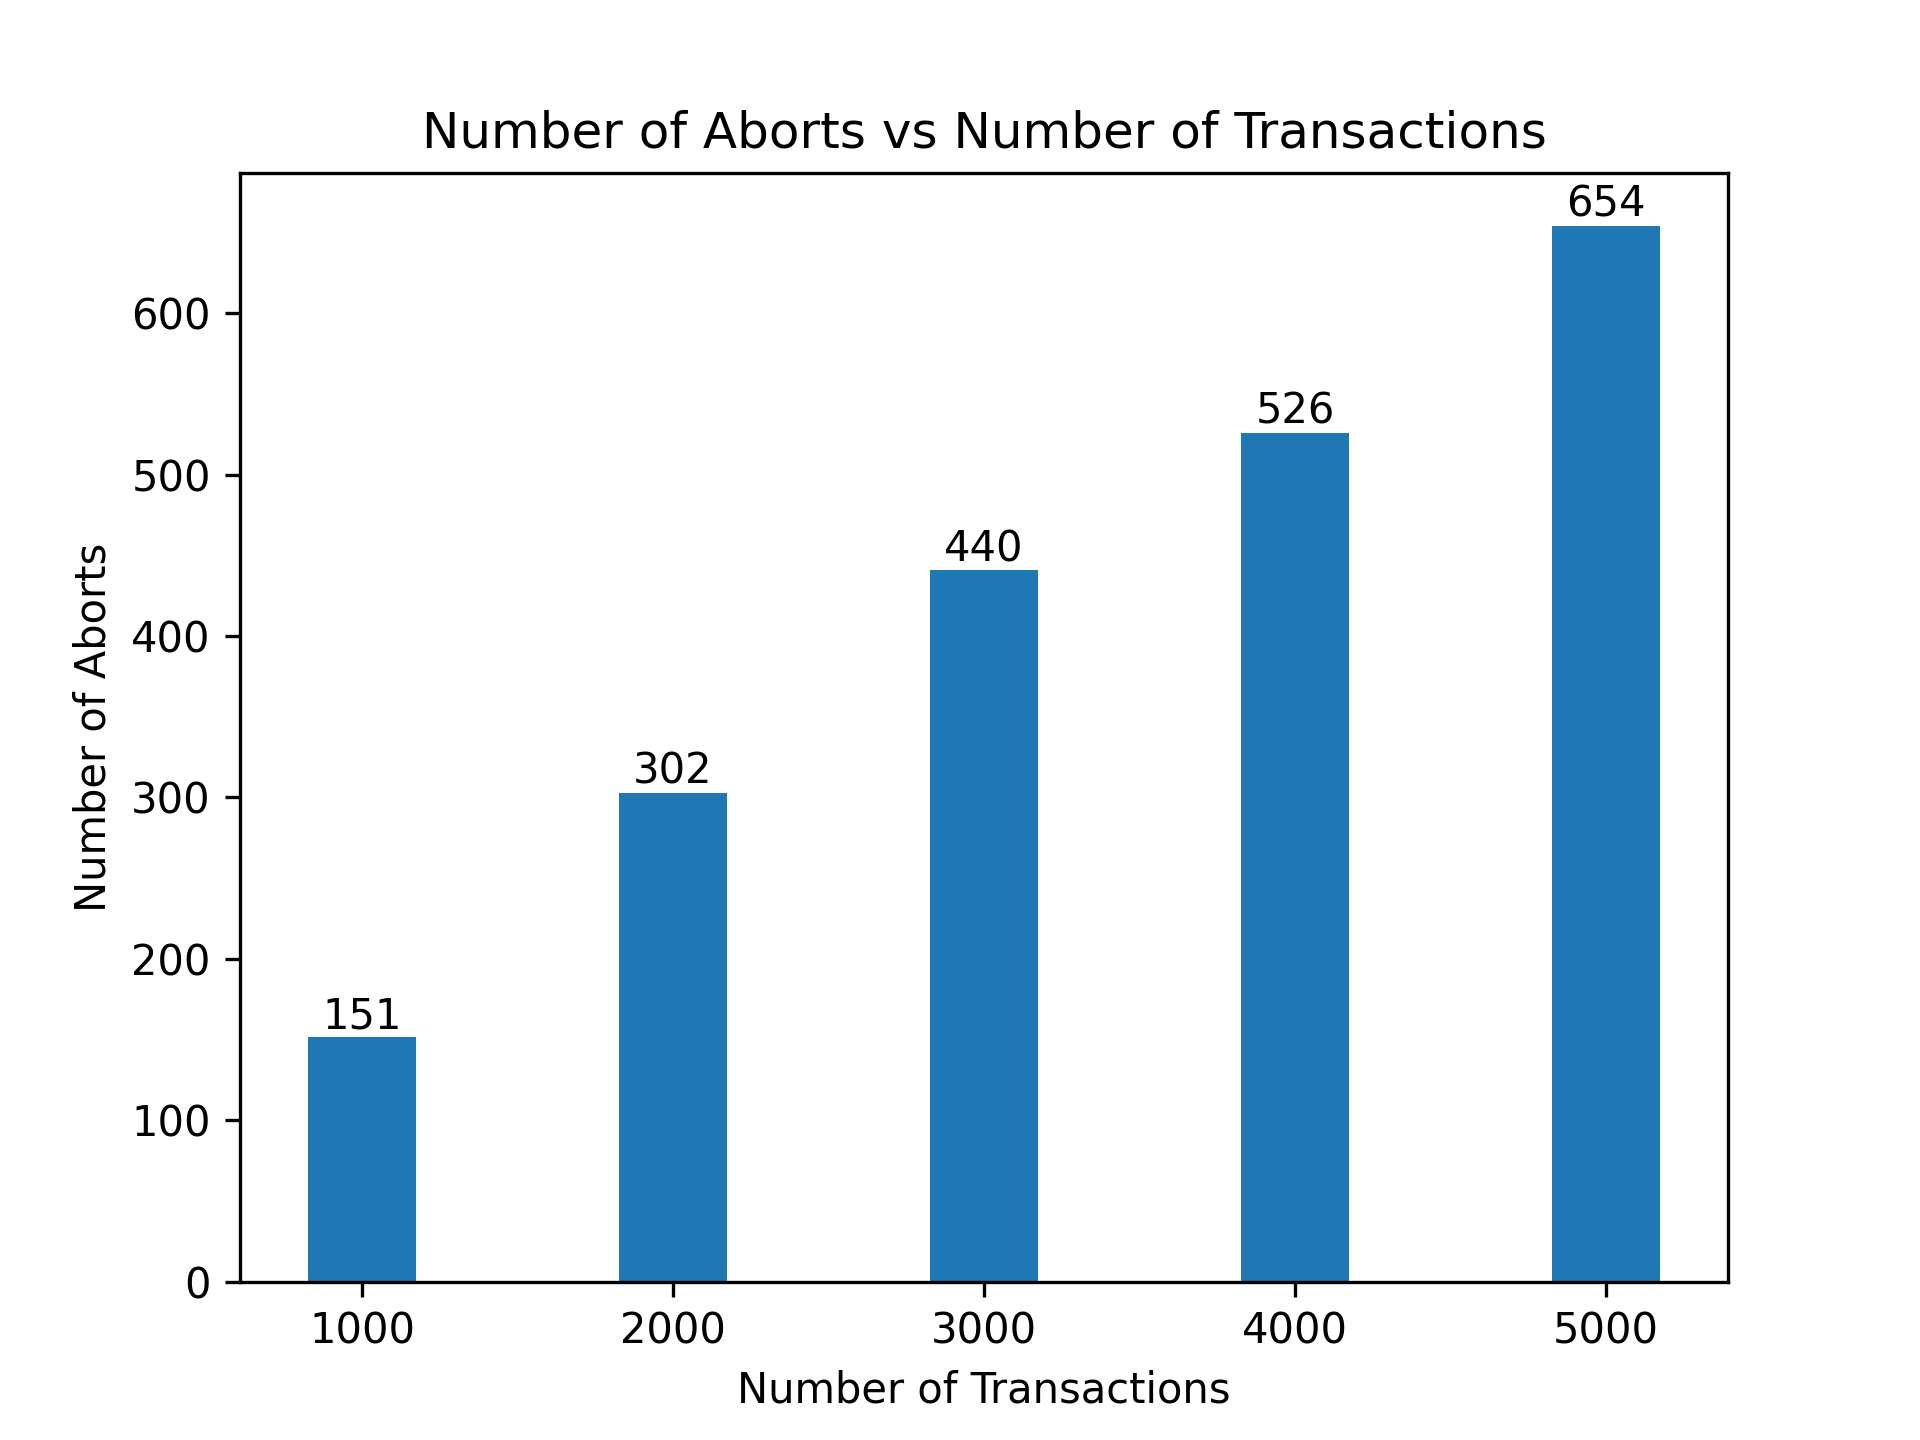
\includegraphics[width=0.8\textwidth]{images/numTrans_vs_Aborts.png}
    % \caption{Number of Aborts vs Number of Transactions}
    % \label{fig:numTrans_vs_Aborts}
    \begin{minipage}
        {0.49\textwidth}
        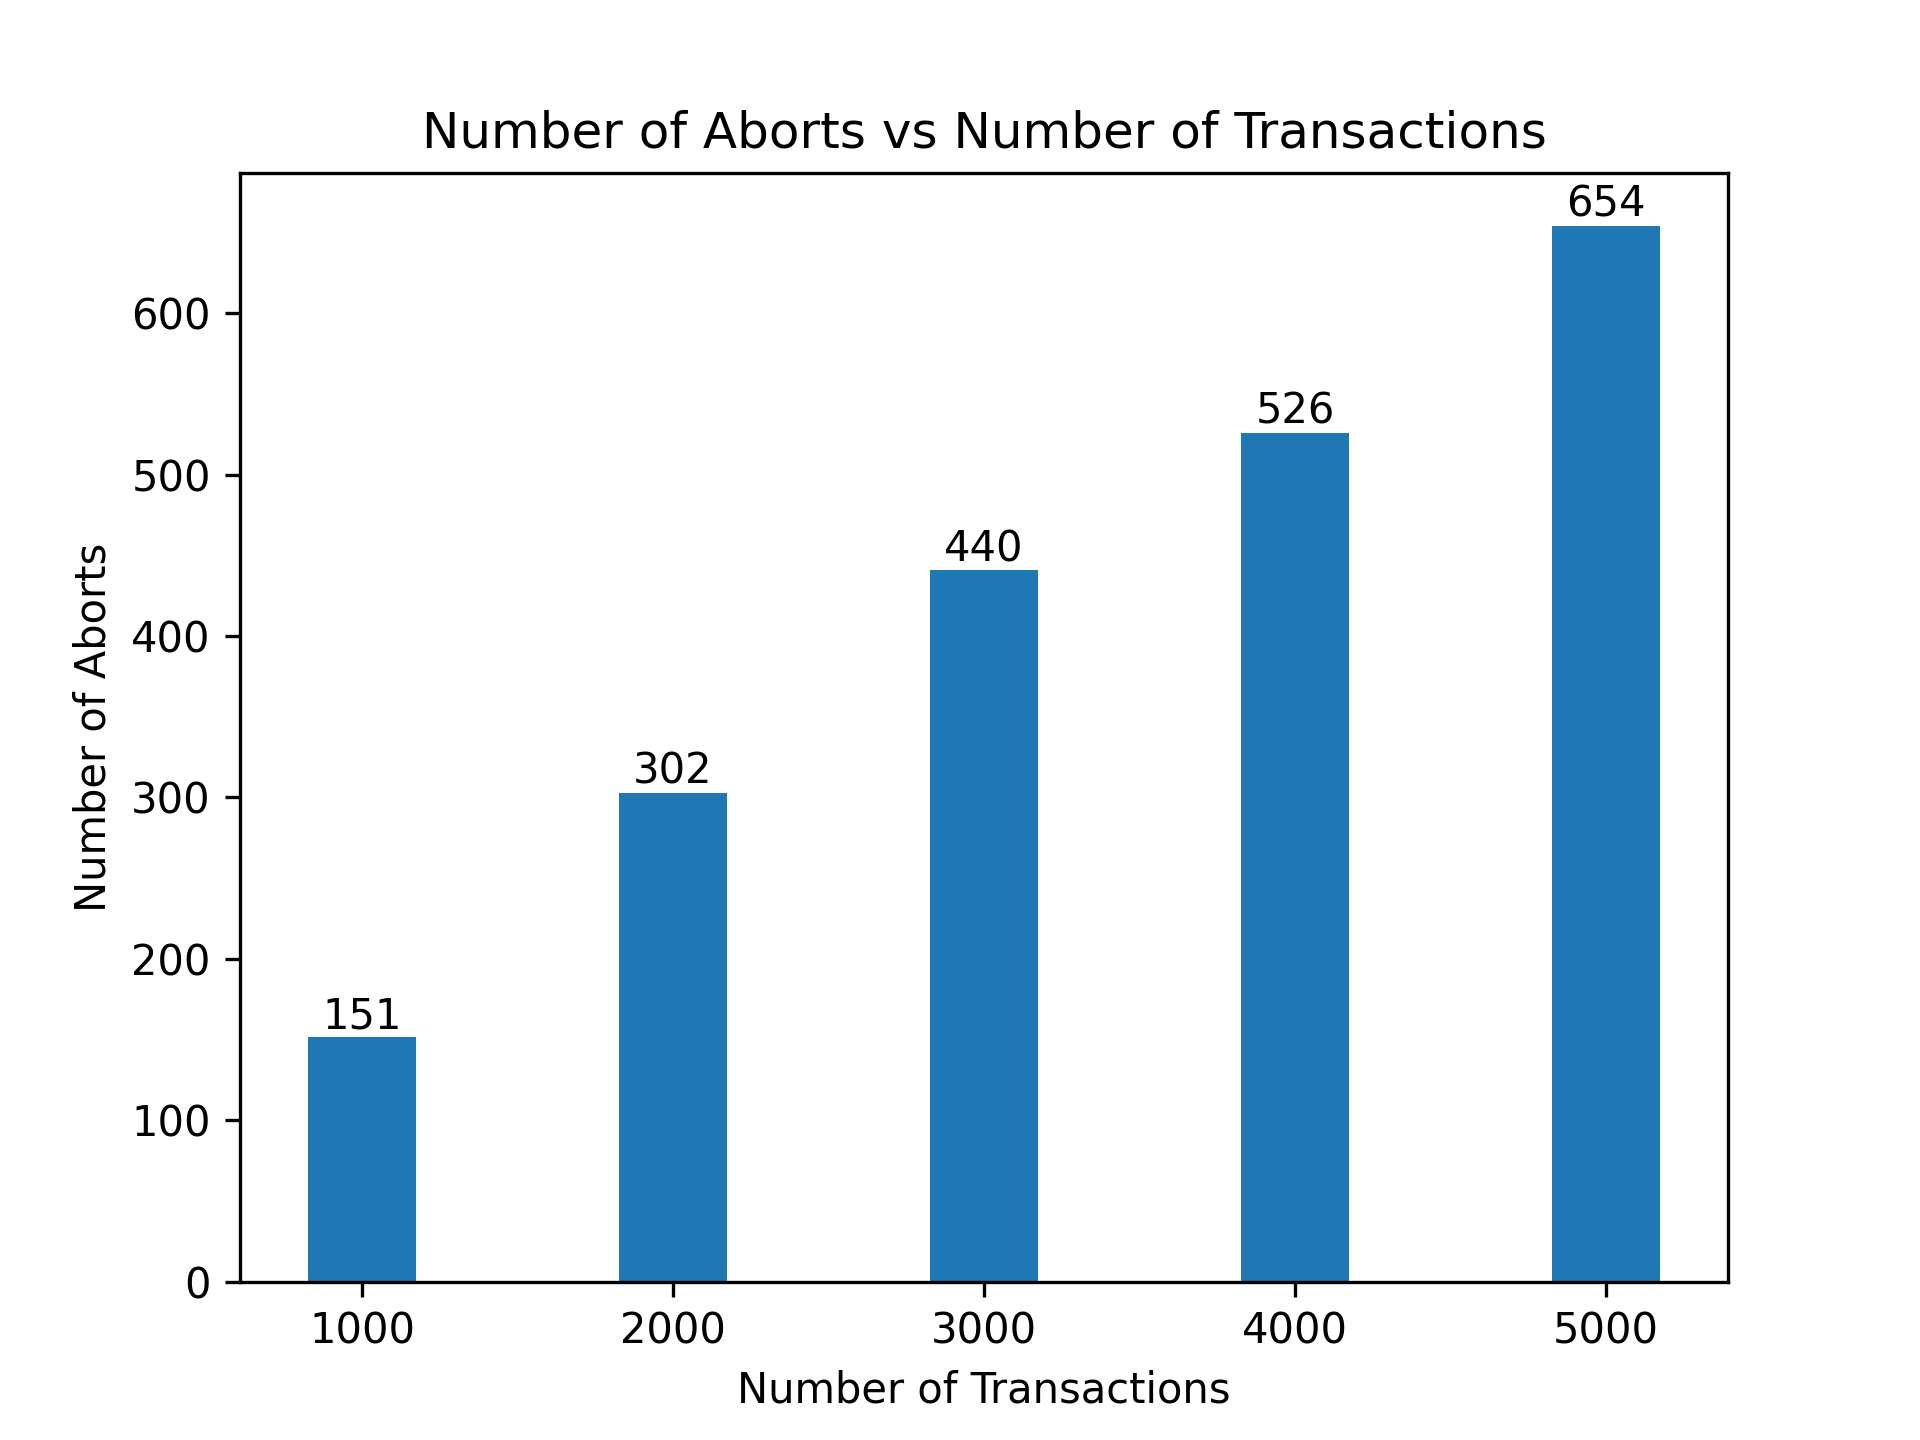
\includegraphics[width=\textwidth]{images/numTrans_vs_Aborts.png}
        \caption{Number of Aborts vs Number of Transactions}
        \label{fig:numTrans_vs_Aborts}
    \end{minipage}
    \hfill
    \begin{minipage}
        {0.49\textwidth}
        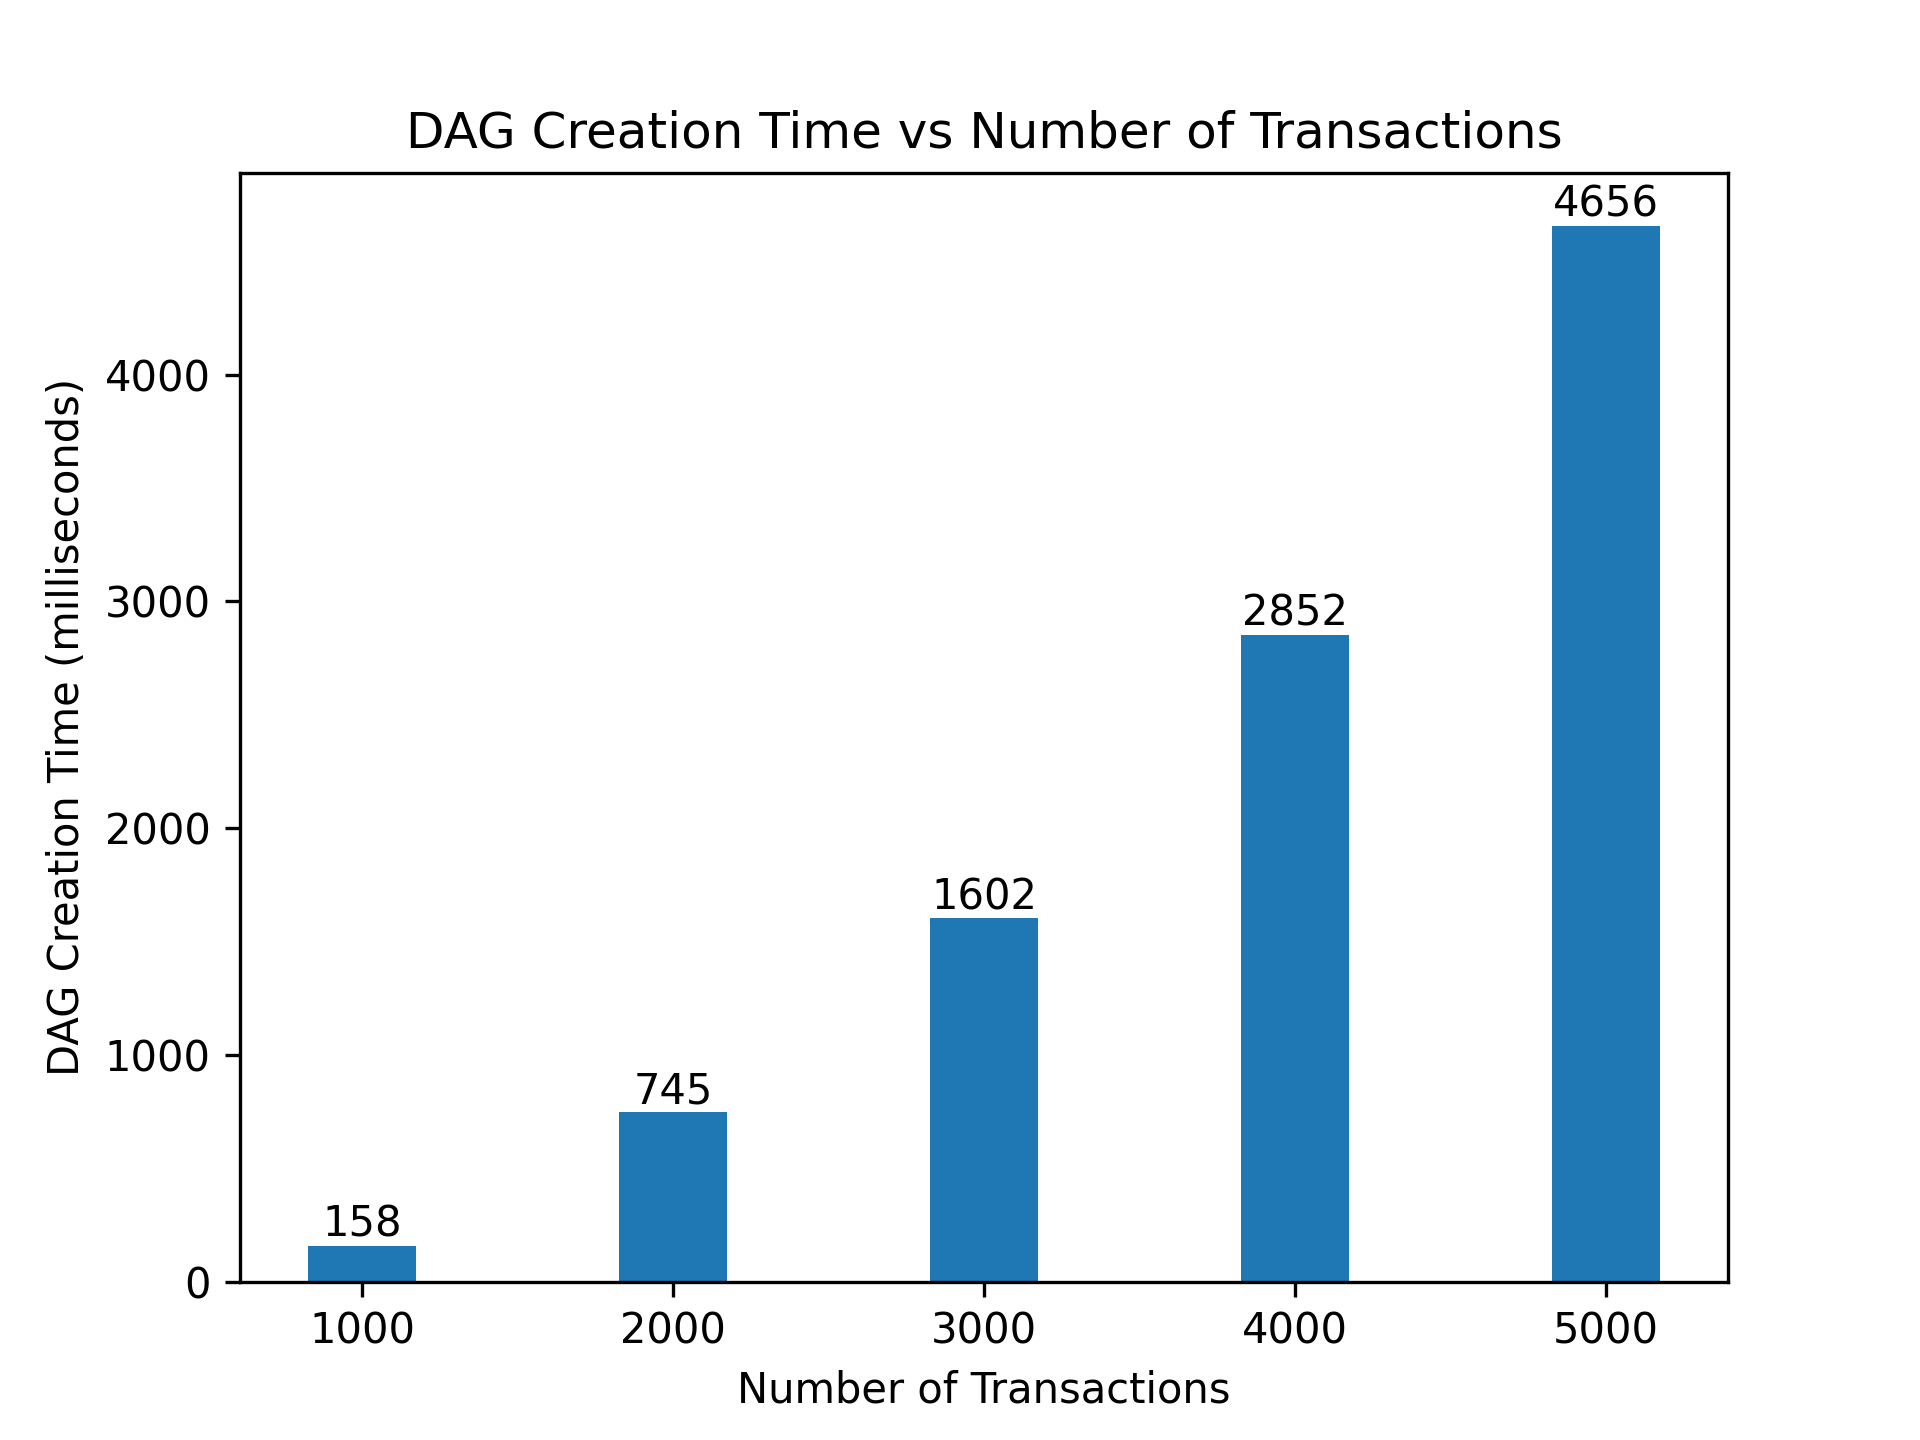
\includegraphics[width=\textwidth]{images/numTrans_vs_DAGCreationTime.png}
        \caption{DAG Creation Time vs Number of Transactions}
        \label{fig:numTrans_vs_DAGCreationTime}
    \end{minipage}
\end{figure}
    

\subsection{Dependency Percentage}
In this experiment dependency percentage is varied from 0\% to 80\% in increments of 20\%.
The number of transactions is kept constant at 3000 and number of threads is kept constant at 16. \\
Figure \ref{fig:dp_vs_Time} shows the execution time vs dependency percentage and Figure \ref{fig:dp_vs_Aborts} shows the number of aborts vs dependency percentage.
Figure \ref{fig:dp_vs_DAGCreationTime} shows the DAG creation time vs dependency percentage.
For DAG time to execute the transactions is taken and reported in figure, DAG creation time is not included.

\begin{itemize}
    \item As dependency percentage increases, the execution time also increases.
    \item Block Pilot performs better than DAG in terms of execution time.
    \item Number of aborts also increases with the dependency percentage.
    \item DAG creation time also increases with the dependency percentage, but the rate of increase decreases as the dependency percentage increases and having almost equal time for 60\% and 80\%.
\end{itemize}

\begin{figure}[h]
    \centering
    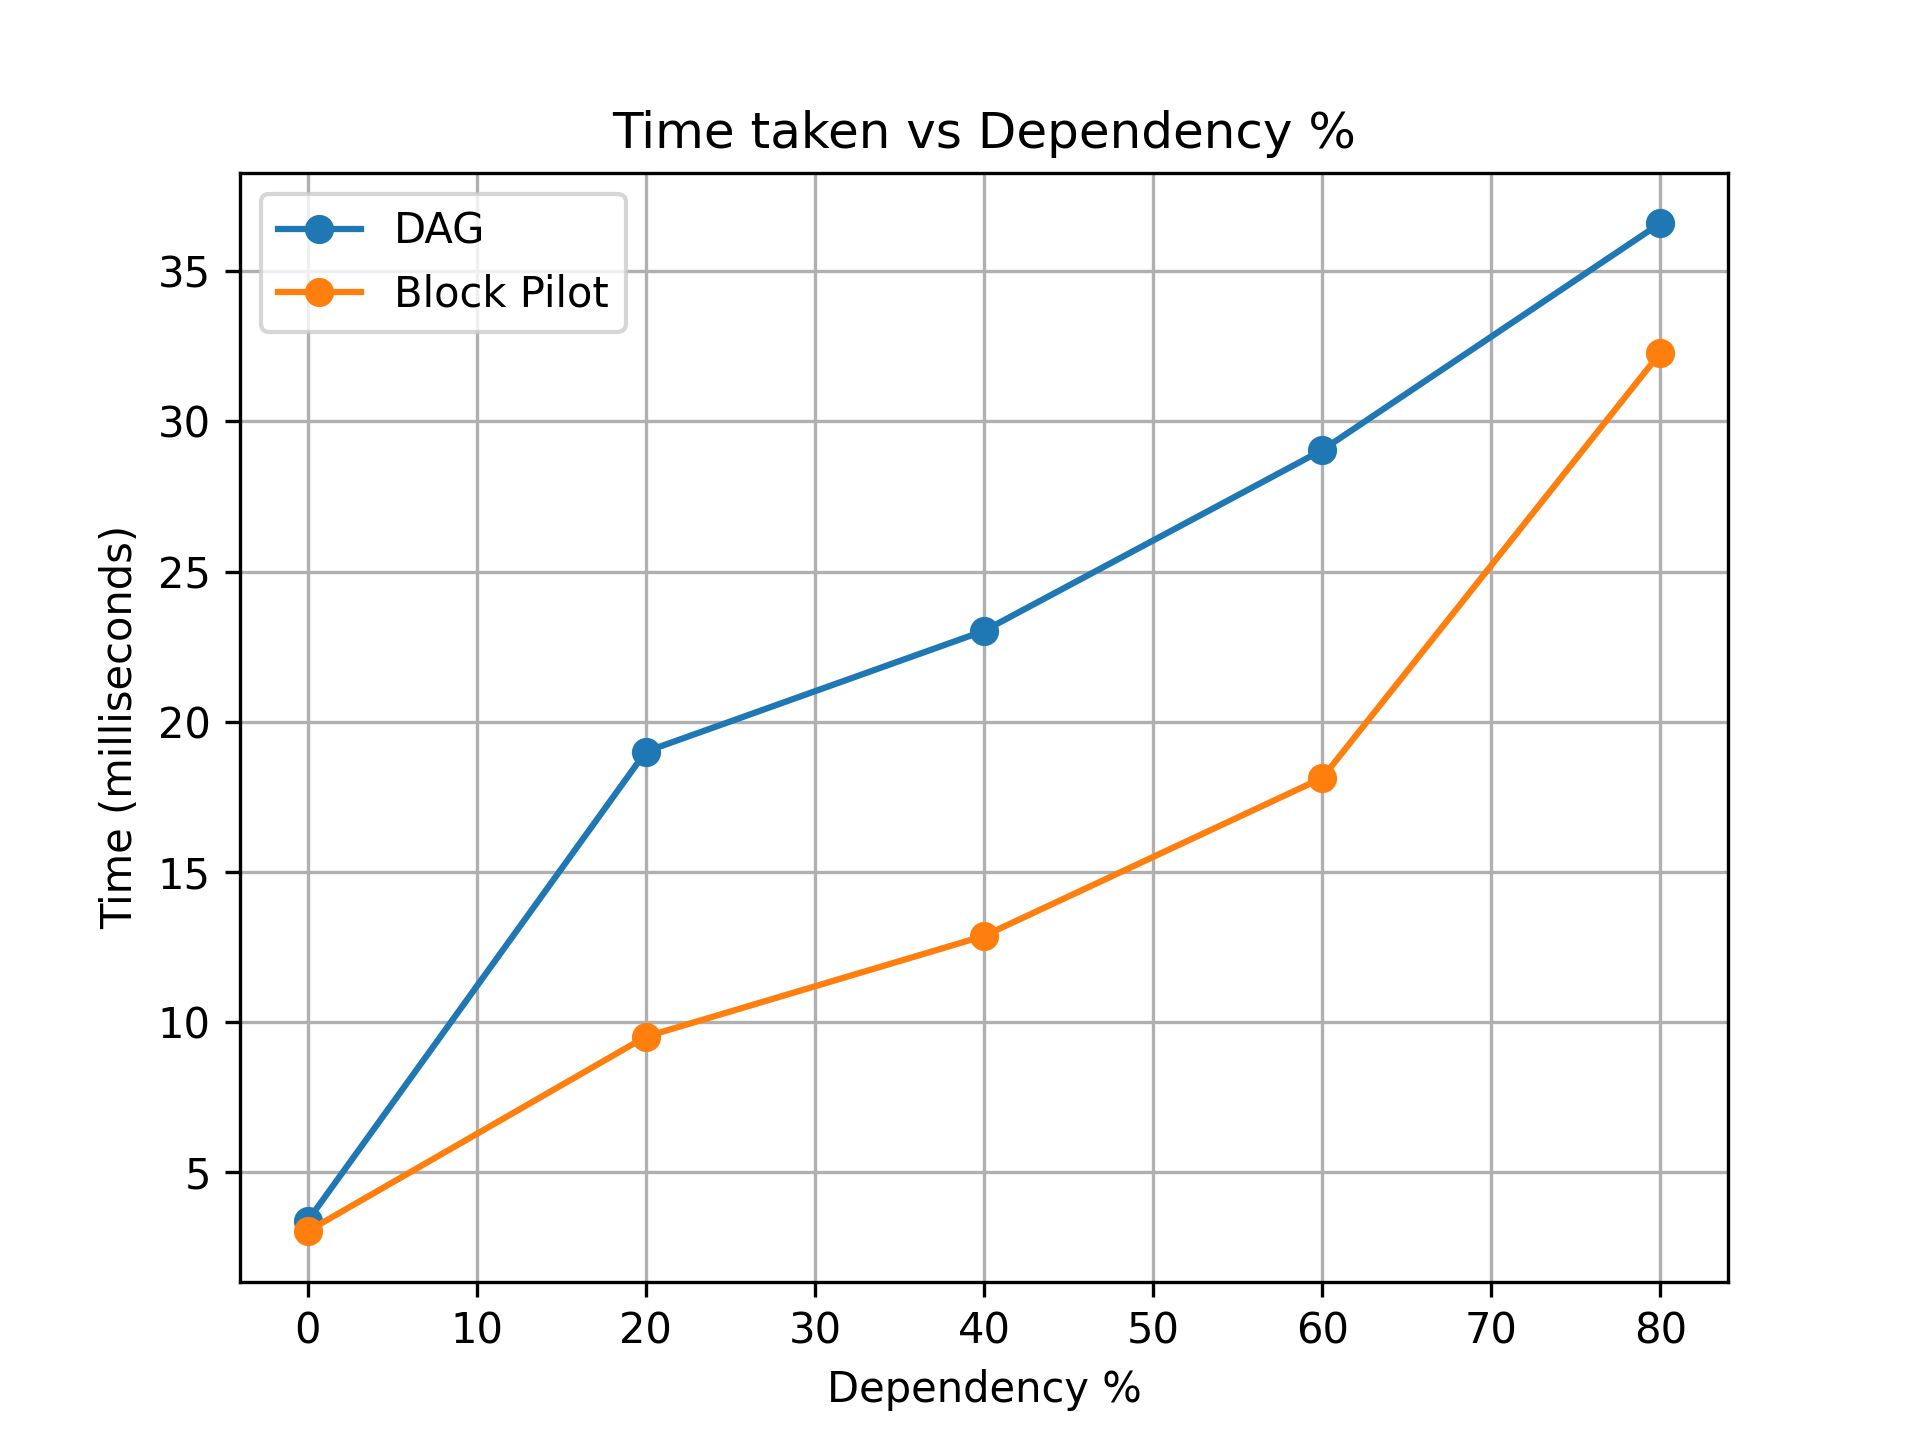
\includegraphics[width=0.8\textwidth]{images/dp_vs_Time.png}
    \caption{Execution Time vs Dependency Percentage}
    \label{fig:dp_vs_Time}
\end{figure}
\begin{figure}[h]
    \centering
    \begin{minipage}
        {0.49\textwidth}
        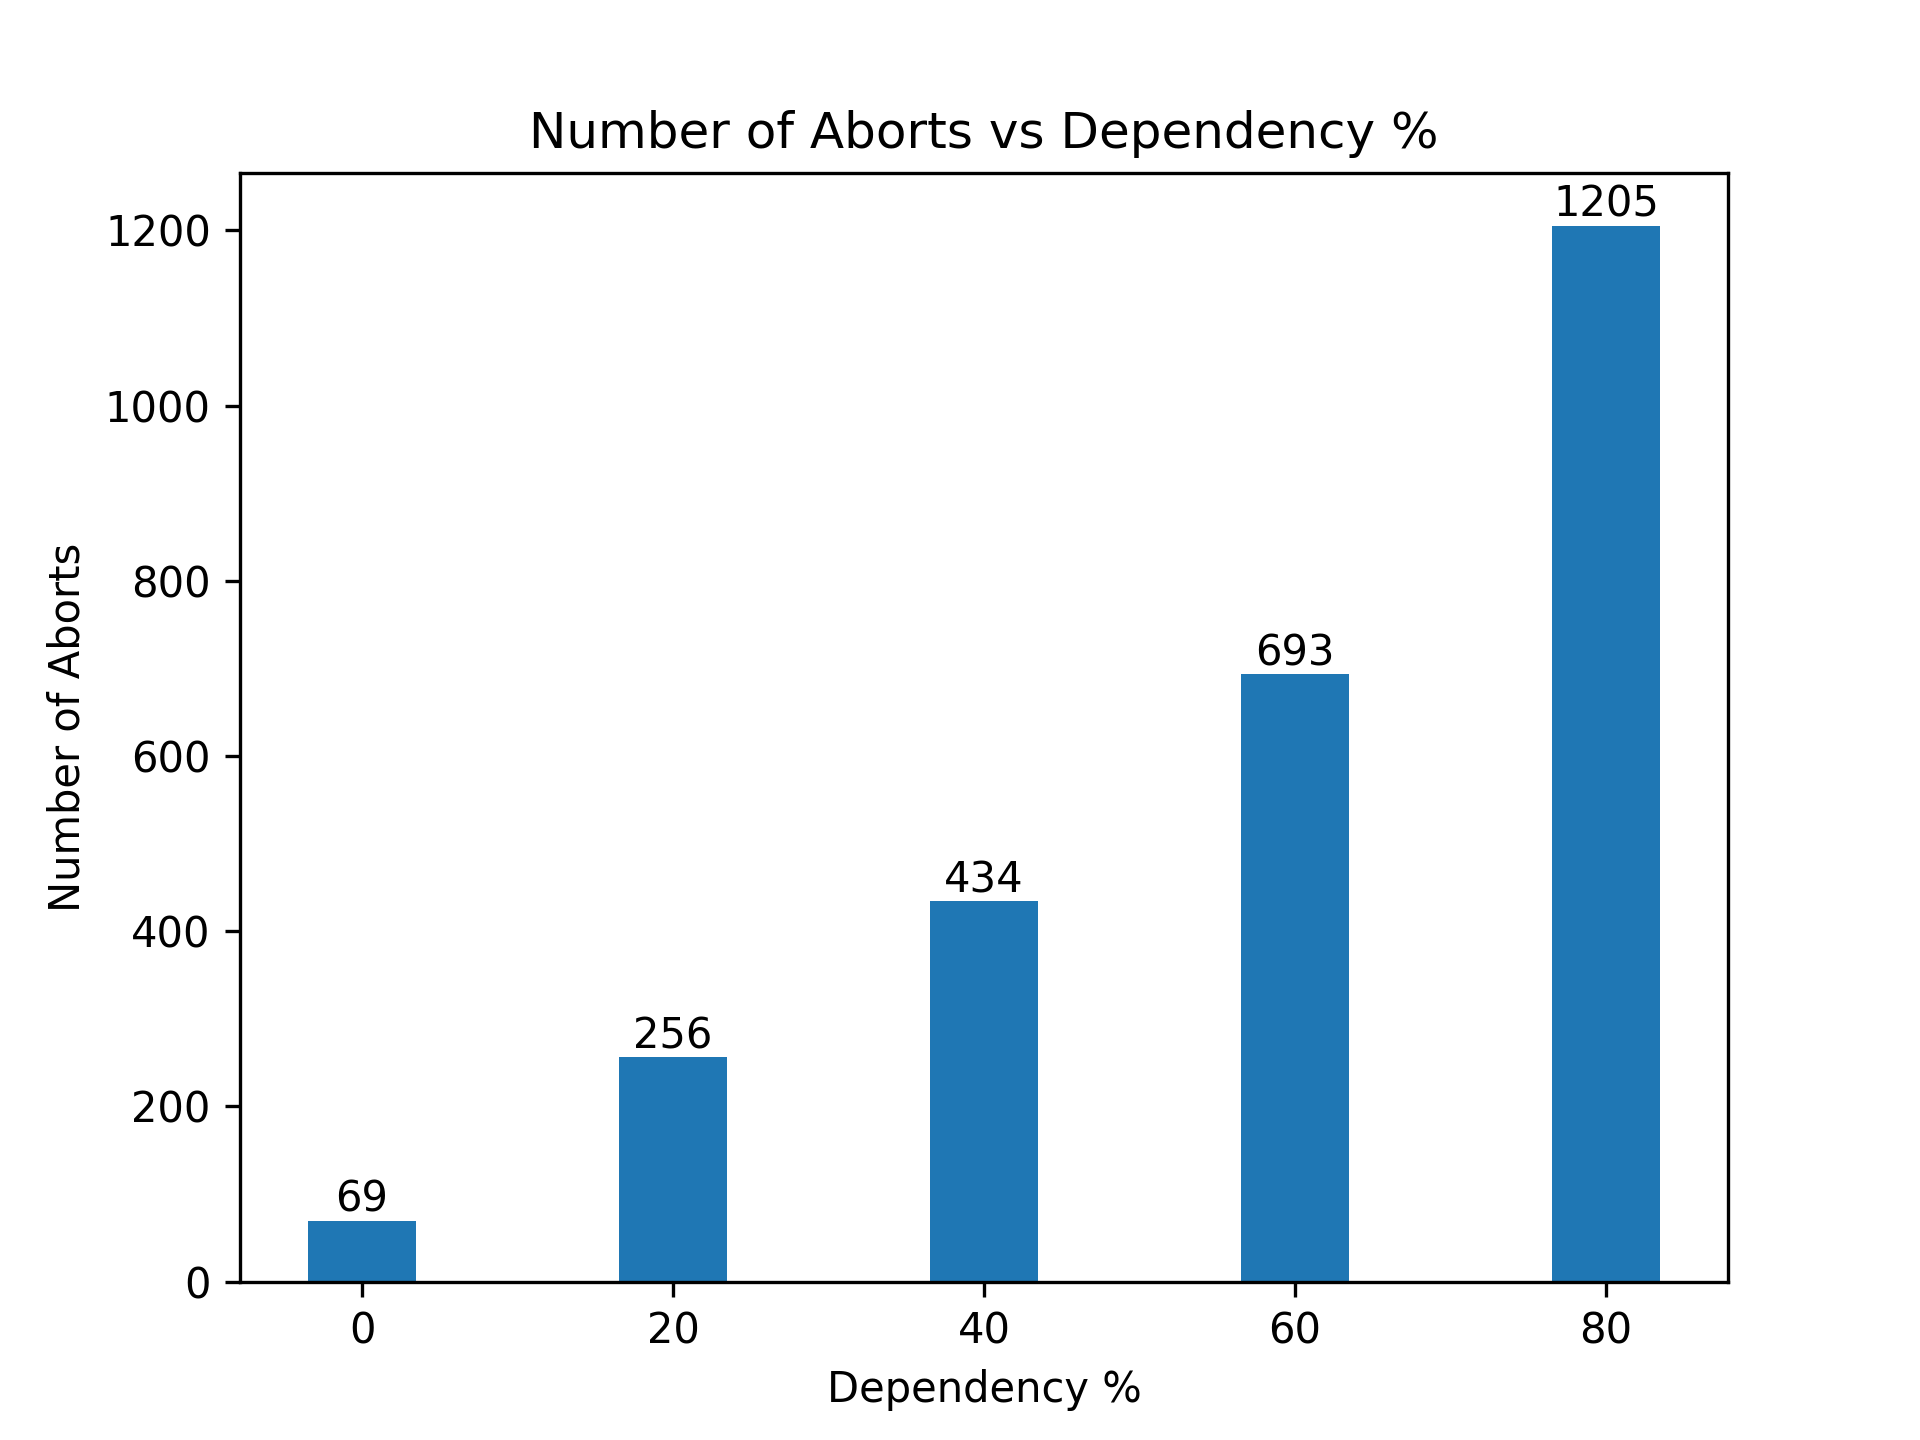
\includegraphics[width=\textwidth]{images/dp_vs_Aborts.png}
        \caption{Number of Aborts vs Dependency Percentage}
        \label{fig:dp_vs_Aborts}
    \end{minipage}
    \hfill
    \begin{minipage}
        {0.49\textwidth}
        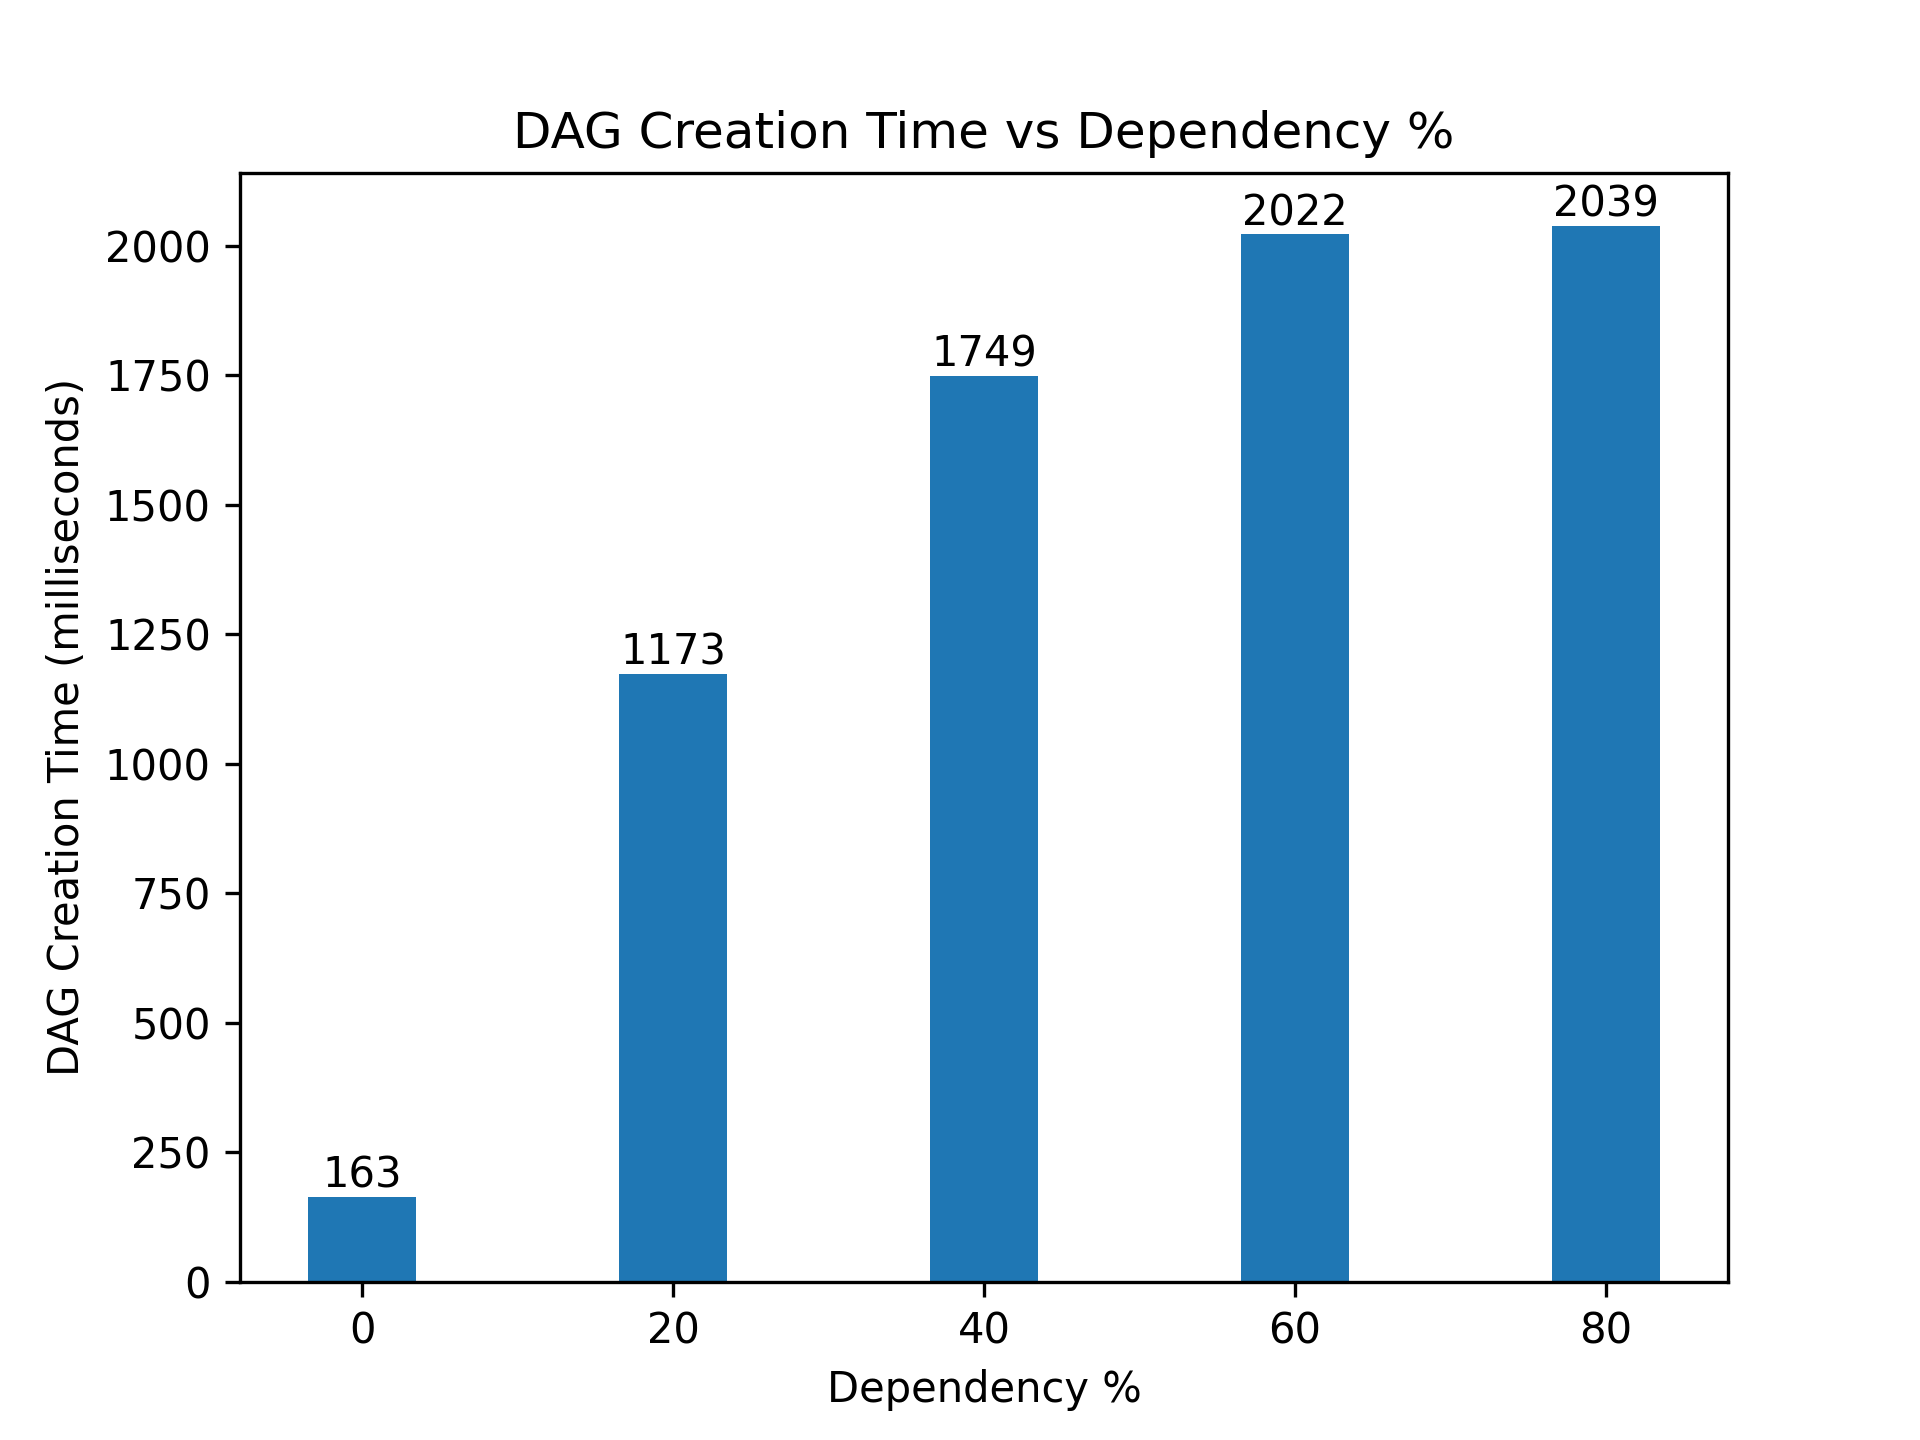
\includegraphics[width=\textwidth]{images/dp_vs_DAGCreationTime.png}
        \caption{DAG Creation Time vs Dependency Percentage}
        \label{fig:dp_vs_DAGCreationTime}
    \end{minipage}
\end{figure}

\subsection{Number of Threads}
In this experiment, the number of threads is varied from 2 to 32 in increments of multiples of 2. 
The number of transactions is kept constant at 3000 and dependency percentage is kept constant at 40\%.
Figure \ref{fig:numThreads_vs_Time} shows the execution time vs number of threads and Figure \ref{fig:numThreads_vs_Aborts} shows the number of aborts vs number of threads.
Figure \ref{fig:numThreads_vs_DAGCreationTime} shows the DAG creation time vs number of threads.
For DAG time to execute the transactions is taken and reported in figure, DAG creation time is not included.
\begin{itemize}
    \item As number of threads increases, the execution first decreases and then increases.
    \item Block Pilot performs better than DAG in terms of execution time.
    \item For Block Pilot as number of threads increases, so number of aborts hence execution time starts increases after 8 threads.
    \item Number of aborts also increases with the number of threads.
    \item DAG creation time decreases with the number of threads, as more threads are available to process the transactions.
\end{itemize}
\begin{figure}[h]
    \centering
    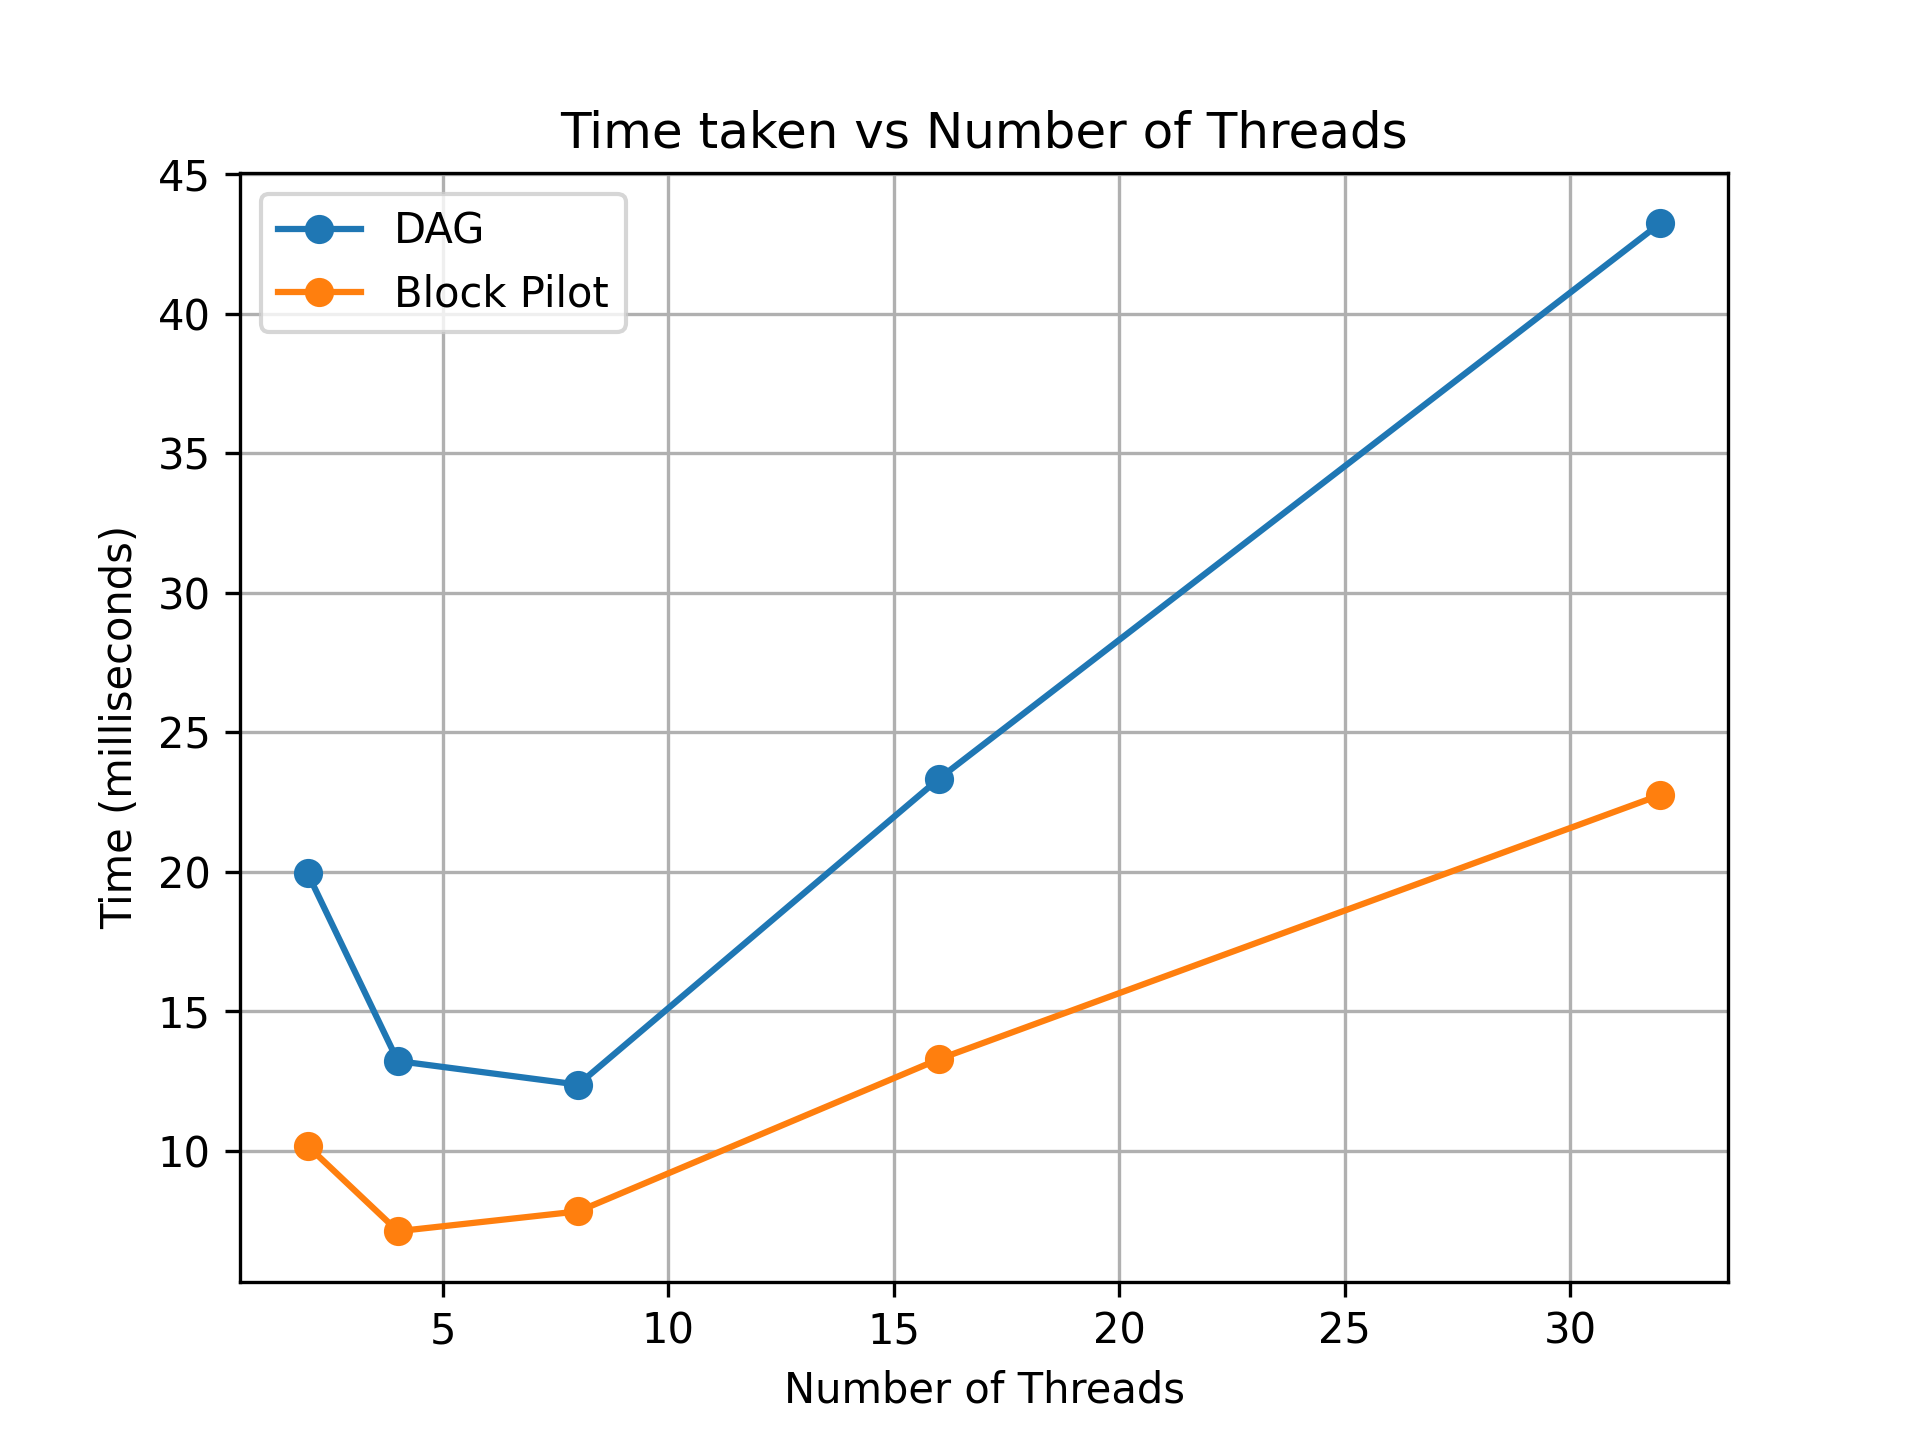
\includegraphics[width=0.8\textwidth]{images/numThreads_vs_Time.png}
    \caption{Execution Time vs Number of Threads}
    \label{fig:numThreads_vs_Time}
\end{figure}

\begin{figure}[h]
    \centering
    \begin{minipage}
        {0.49\textwidth}
        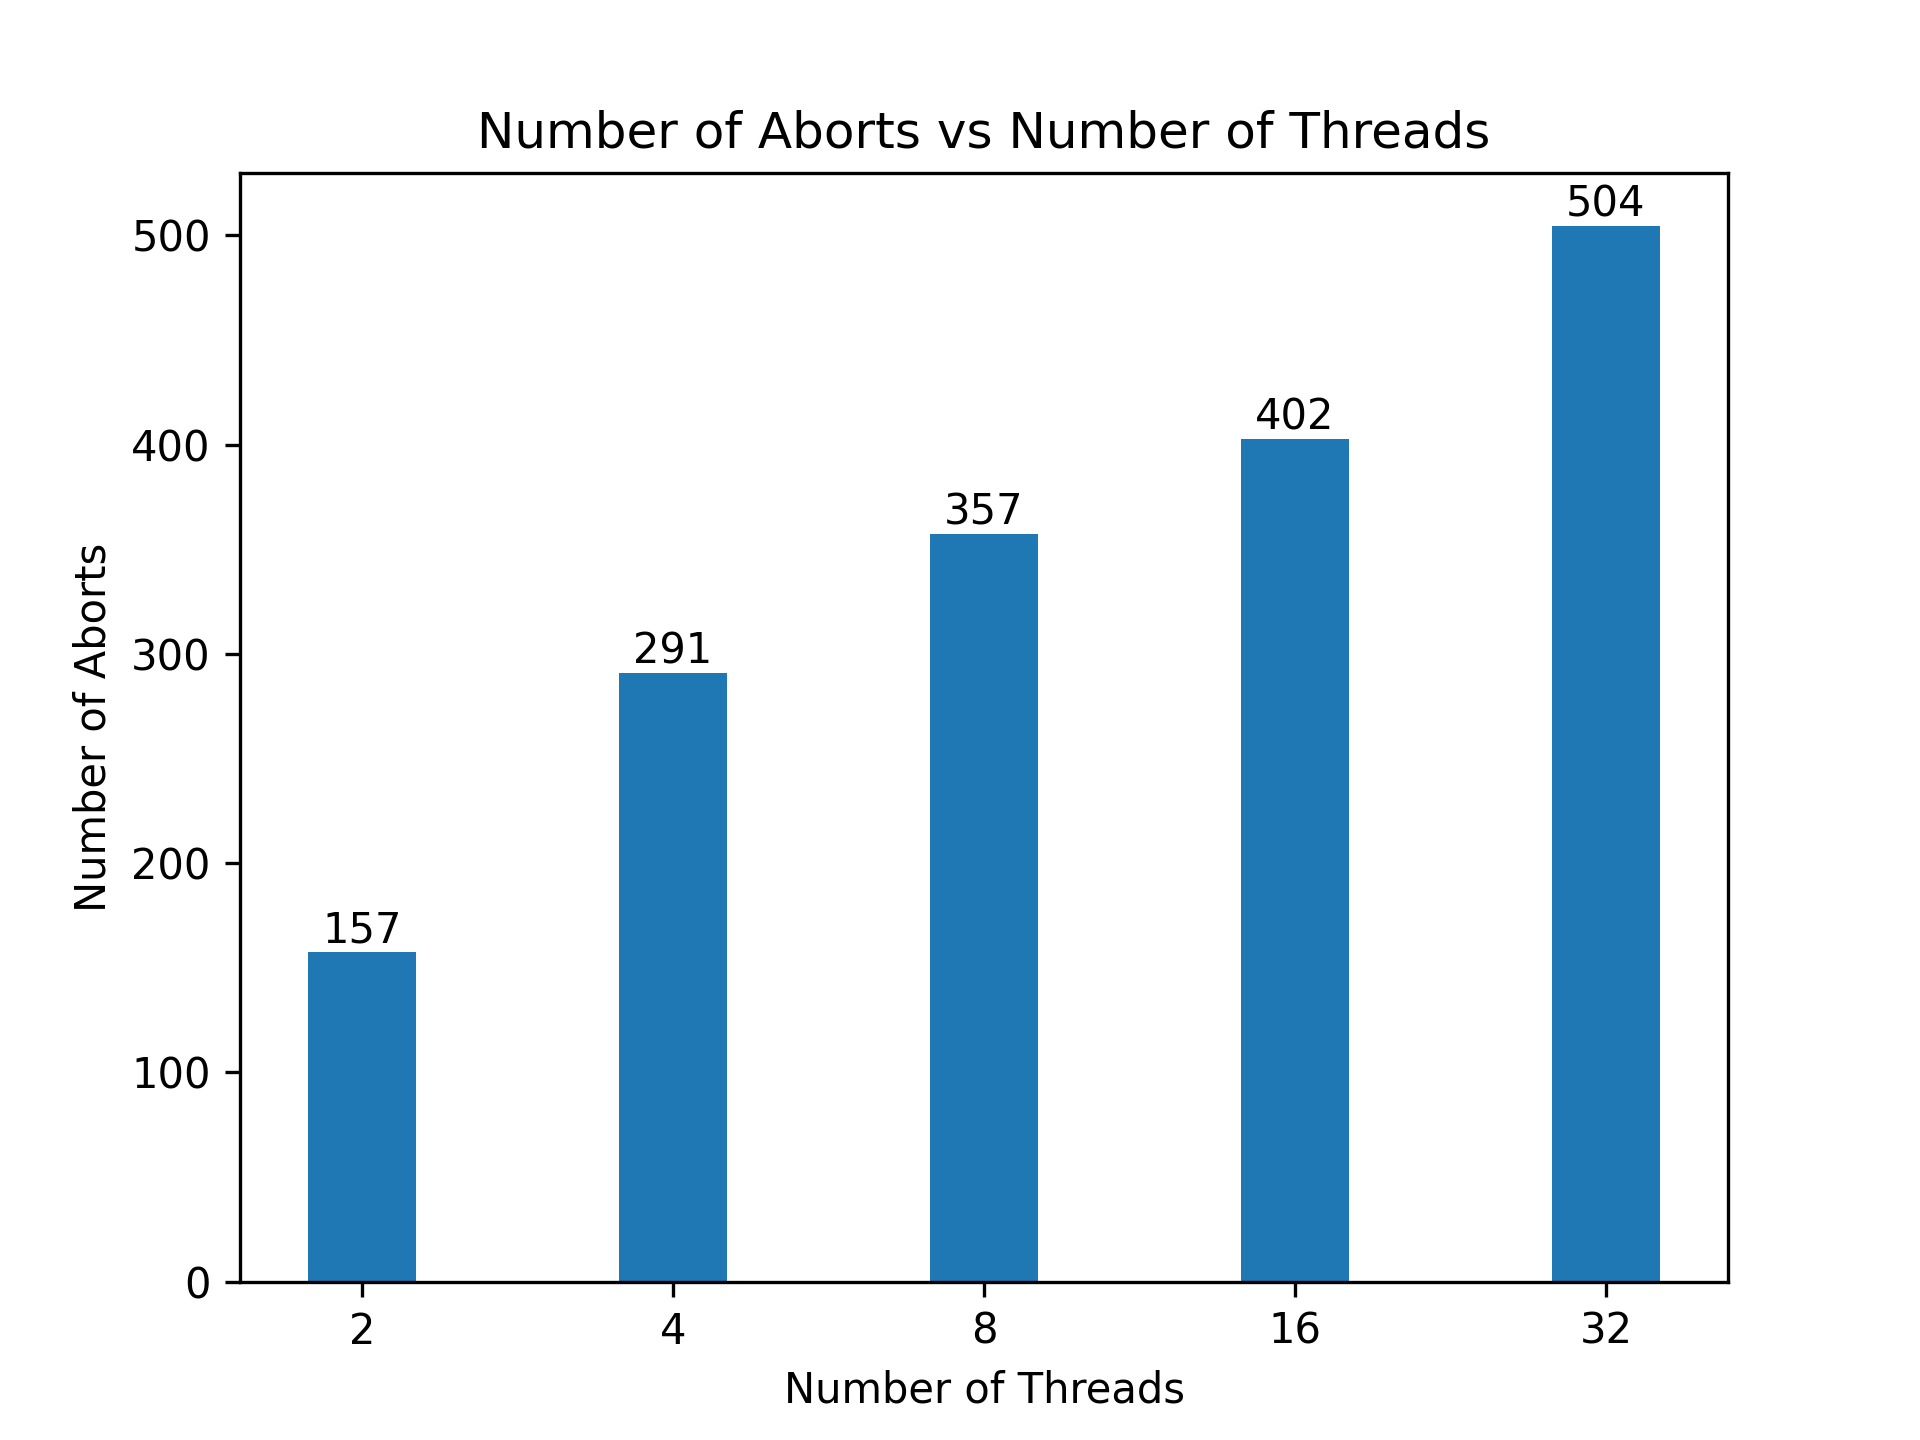
\includegraphics[width=\textwidth]{images/numThreads_vs_Aborts.png}
        \caption{Number of Aborts vs Number of Threads}
        \label{fig:numThreads_vs_Aborts}
    \end{minipage}
    \hfill
    \begin{minipage}
        {0.49\textwidth}
        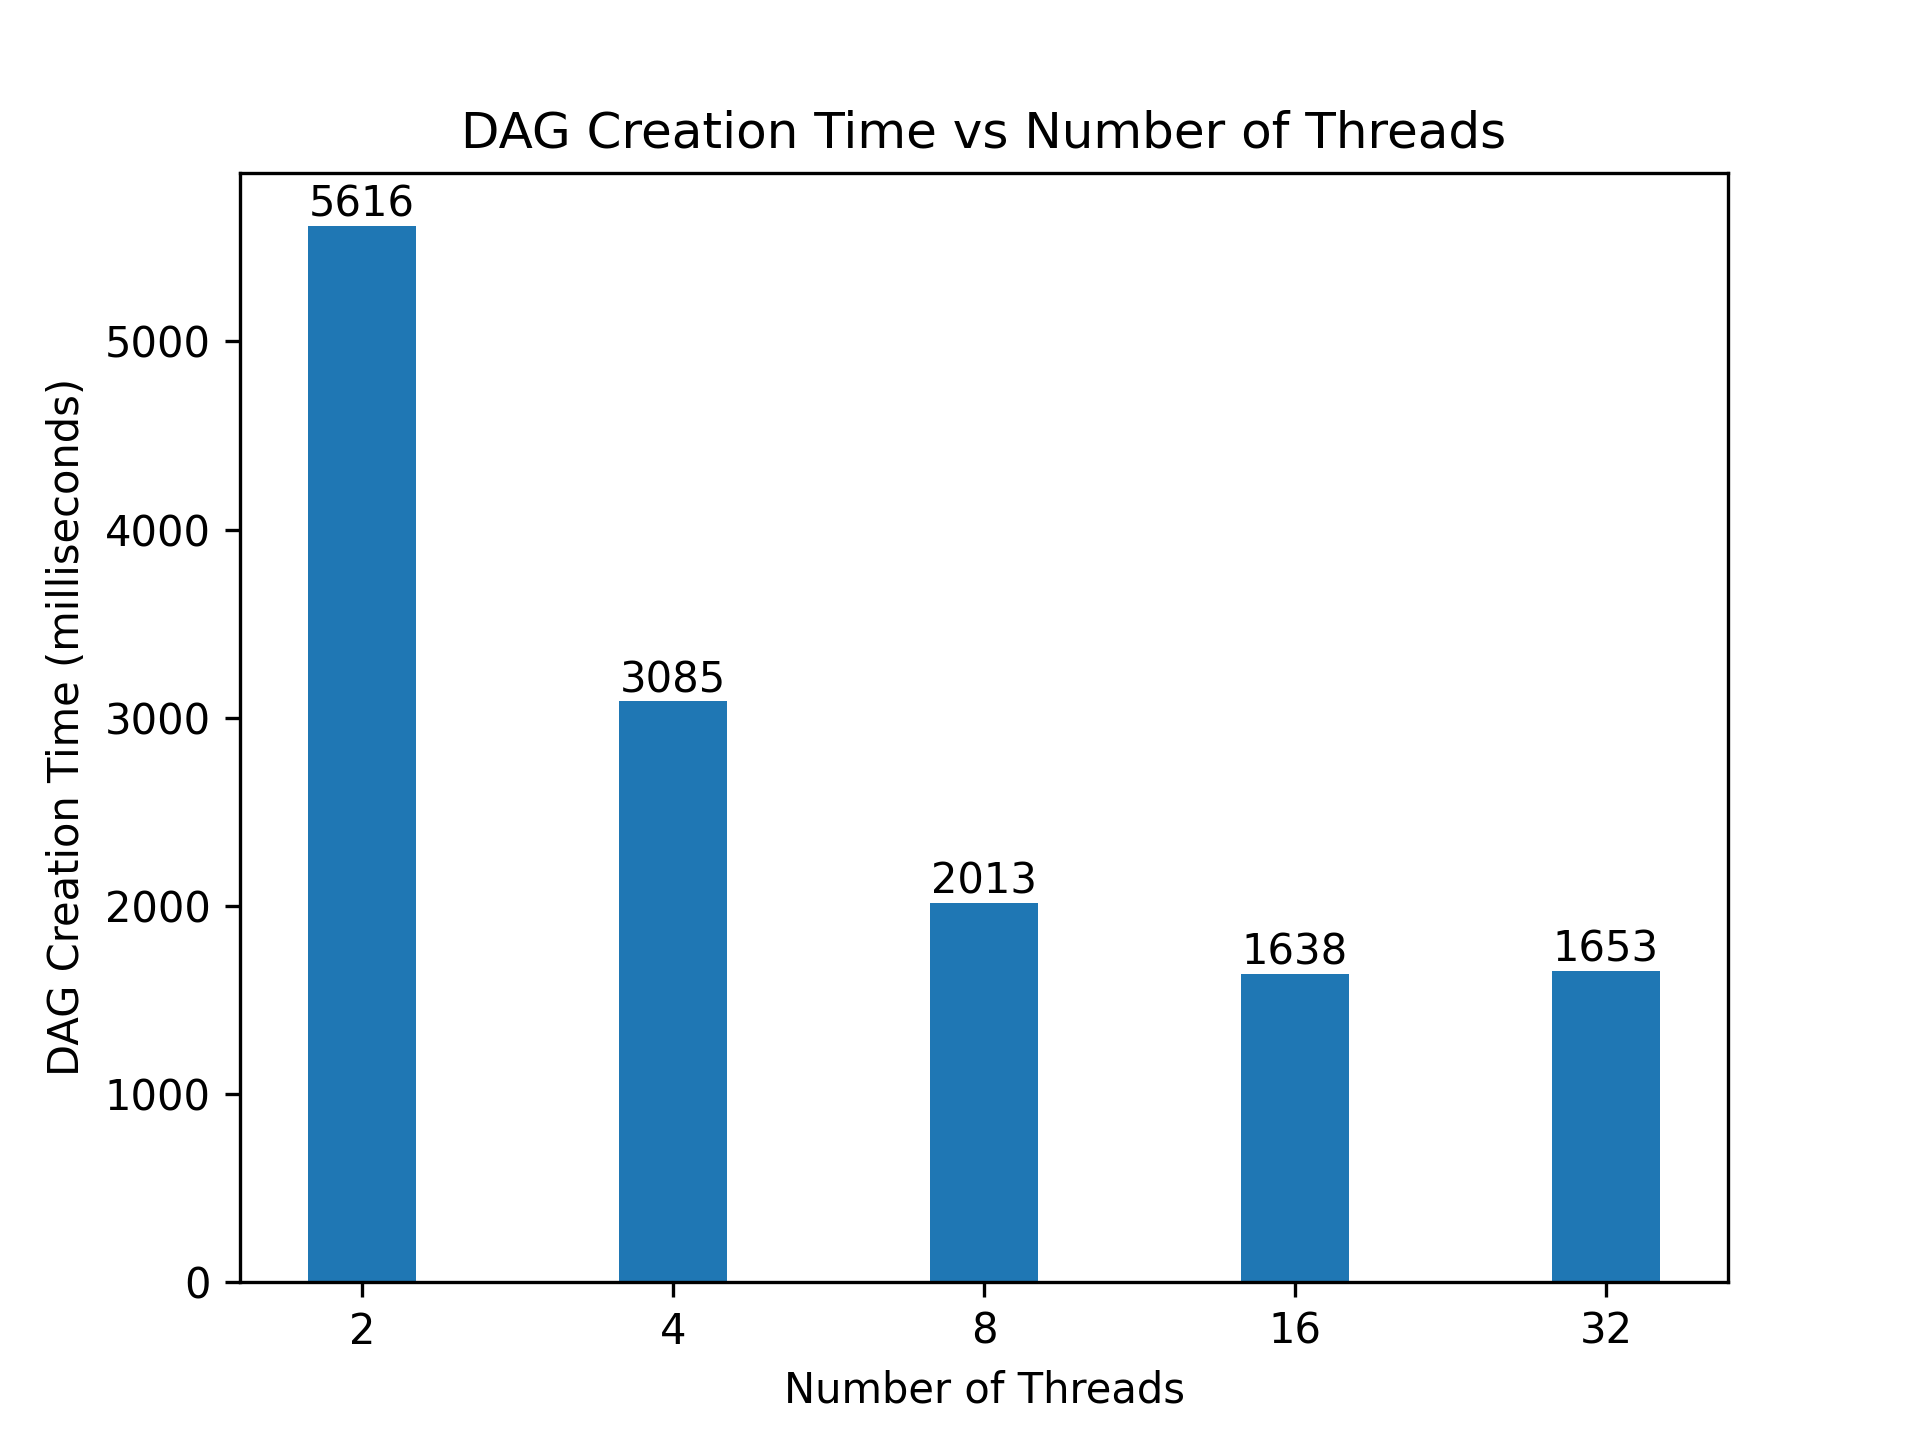
\includegraphics[width=\textwidth]{images/numThreads_vs_DAGCreationTime.png}
        \caption{DAG Creation Time vs Number of Threads}
        \label{fig:numThreads_vs_DAGCreationTime}
    \end{minipage}
\end{figure}

\section{Observation and Conclusion}
In our experiments, we observed that:
\begin{itemize}
    \item BlockPilot consistently outperformed the DAG framework in terms of execution time across all experiments.
    \item As the number of transactions and dependency percentage increased, the execution time and number of aborts also increased.
    \item The DAG creation time increased with the number of transactions and dependency percentage, but decreased with the number of threads.
    \item The number of aborts increased with the number of transactions, dependency percentage, and number of threads for BlockPilot
\end{itemize}
In conclusion, the BlockPilot framework demonstrates superior performance in parallel execution of smart contract transactions compared to the DAG framework. The results indicate that the choice of concurrency control and scheduling mechanisms significantly impacts the efficiency of transaction processing in blockchain systems. 
DAG framework can be used when there is no acceptance for aborts in the system, as it does not abort any transactions.
However, it is important to note that the DAG framework may not be suitable for all scenarios, especially when the number of transactions is large and the dependency percentage is high. In such cases, the BlockPilot framework may be a better choice due to its ability to handle conflicts and aborts more efficiently.


\section{References}

\begin{enumerate}
    \item Haowen Zhang, Jing Li, He Zhao, Tong Zhou, Nianzu Sheng, and Hengyu Pan. \textit{BlockPilot: A Proposer-Validator Parallel Execution Framework for Blockchain}. In 52nd International Conference on Parallel Processing (ICPP), 2023. DOI: \href{https://doi.org/10.1145/3605573.3605621}{10.1145/3605573.3605621}.
    \item Parwat Singh Anjana et al. \textit{An Efficient Framework for Optimistic Concurrent Execution of Smart Contracts}. In EuroMicro PDP, 2019. DOI: \href{https://doi.org/10.1007/978-3-031-39698-4_13}{10.1007/978-3-031-39698-4\_13}.
\end{enumerate}

\end{document}